%%%%%%%%%%%%%%%%%%%%%%%%%%%%%%%%%%%%%%%%%%%%%%%%%%%%%%%%%%%%%%%%%%%%%%%%%%%%%
% Instruction tuning and preference optimisation of an 8B model.
% NeurIPS 2026 formatting, [preprint] option.
% Compile:  latexmk -pdf tech_report.tex
% Figures:  python make_figures.py   (writes figures/*.pdf from runs/)
%%%%%%%%%%%%%%%%%%%%%%%%%%%%%%%%%%%%%%%%%%%%%%%%%%%%%%%%%%%%%%%%%%%%%%%%%%%%%
\documentclass{article}

% numeric citations, as in the NeurIPS reference style; must precede the style
% file, which loads natbib
\PassOptionsToPackage{numbers, compress}{natbib}
\usepackage[preprint]{neurips_2026}

\usepackage[utf8]{inputenc}
\usepackage[T1]{fontenc}
\usepackage{hyperref}
\usepackage{url}
\usepackage{booktabs}
\usepackage{multirow}
\usepackage{amsfonts}
\usepackage{amsmath}
\usepackage{amssymb}
\usepackage{microtype}
\usepackage{graphicx}

\newcommand{\lc}{\textsc{lc}}
\newcommand{\sft}{\textsc{sft}}
\newcommand{\dpo}{\textsc{dpo}}

% Two lines, each deliberately under the ~50-character width at this size: a line
% that overflows wraps again and leaves a single word stranded below it.
\title{Instruction Tuning and Preference Optimization:\\
Capability Trade-offs and Judge Dependence}

\author{%
  Yi Hou \\
  University of Chinese Academy of Sciences \\
  Beijing, China \\
  \texttt{houyi25@mails.ucas.ac.cn} \\
}

\begin{document}

\maketitle

\begin{abstract}
We fine-tune an 8B base language model in two stages --- supervised instruction
tuning on 228{,}743 examples, then direct preference optimization on 49{,}326
human preference pairs --- and evaluate it on knowledge (MMLU), reasoning
(GSM8K), open-ended quality (AlpacaEval) and safety (SimpleSafetyTests).
Three results stand out. First, the apparent knowledge gain from instruction
tuning (+7.0 points on MMLU) is mostly a change in \emph{answer format}: the base
model fails to produce a parseable answer on 9.8\% of items under the
instruction-tuned prompt template and the fine-tuned model fails on none, while
its answers shrink from 353 to 27 characters. The same brevity costs 4.5 points
on GSM8K, where the dropped text was the reasoning. Second, preference
optimization partly reverses this: it restores GSM8K above the base model at the
cost of both MMLU and format compliance. Third, and most consequentially,
\emph{the judge dominates the number}. The same model outputs scored by four
judges of different capability yield AlpacaEval winrates spanning 3.8\% to 33.2\%;
a locally served 8B judge rates every model 5--8$\times$ higher than three
frontier APIs and exhibits 10--25$\times$ position bias against their
1.0--1.8$\times$. The ordering of our three models survives across the three
frontier judges and under the benchmark's own length-controlled metric, but not
across a weak judge. We report the length-controlled winrate alongside the raw
one throughout.
\end{abstract}

\section{Introduction}

Post-training a base language model typically proceeds in two stages: supervised
instruction tuning, which teaches the model to follow instructions and adopt an
answer format, and preference optimization, which shifts the model toward answers
annotators prefer. Both are standard, and the question worth asking about a
particular pair of them is not whether they work but \emph{what they change} ---
which capabilities move, in which direction, and how much of the measured
movement is the model rather than the instrument.

This report studies that question at the 8B scale, where a full pipeline is
affordable and every number can be traced to a run. We take an 8B base model,
apply LoRA supervised fine-tuning on 228{,}743 instructions, then LoRA DPO on
49{,}326 human preference pairs, and evaluate the base, the fine-tuned and the
preference-tuned models on four axes: MMLU \citep{hendrycks2021mmlu}, GSM8K
\citep{cobbe2021gsm8k}, AlpacaEval \citep{li2023alpacaeval} and SimpleSafetyTests
\citep{vidgen2024sst}.

Our contributions are:

\begin{itemize}
\item A two-stage pipeline trained end to end under a fixed compute budget, with
      throughput, memory and loss records reported alongside the evaluation, so
      the cost of each result is legible.
\item Evidence that the instruction-tuning MMLU gain at this scale is dominated
      by format compliance rather than knowledge, and that the corresponding loss
      on GSM8K comes from the same shortening.
\item A judge study: the same 805 AlpacaEval predictions scored by four judges of
      different capability and family, which quantifies how much of a
      judge-scored number is the judge. We find the absolute level is not robust
      at all, position bias scales inversely with judge capability, and --- the
      part that matters for practice --- the model \emph{ordering} survives
      across frontier judges but not across a weak one.
\end{itemize}

\section{Setup}

\subsection{Models, data and hardware}

The base model is Llama-3.1-8B. Instruction tuning uses a 228{,}743-example
single-turn mixture drawn from UltraChat-200K \citep{ding2023ultrachat} and the
SafetyTunedLlamas preference set, packed into 512-token sequences (120M tokens in
the training split). Preference optimization uses Anthropic's HH preference data
\citep{bai2022hh}: of 160{,}800 rows across the four released splits, dropping
multi-turn conversations and rows whose two branches do not share a prompt leaves
49{,}326 comparable pairs.

Both stages fit LoRA adapters \citep{hu2021lora} (rank 16, $\alpha=32$, dropout
0.05, all attention and MLP projections) rather than full parameters: full
fine-tuning of an 8B model in fp32 Adam needs roughly 96\,GB of optimizer state
alone, which does not fit the 48\,GB cards this work ran on. LoRA does not make
the step cheaper --- the forward and backward still traverse every parameter ---
it only makes the optimizer affordable.

Everything ran on a single shared A6000 (48\,GB) with four other tenants.

\subsection{Supervised fine-tuning}

\begin{table}[t]
\centering
\caption{Supervised fine-tuning. Throughput is the median over the run; the run
stopped at 68\% of one epoch because the loss had flattened, not because of a
failure.}
\label{tab:sft}
\small
\begin{tabular}{ll}
\toprule
examples / tokens & 228{,}743 / 120M \\
effective batch & 32 (8 micro-batches $\times$ 4 accumulation steps) \\
sequence length & 512 \\
optimizer & AdamW, peak lr $2\times10^{-4}$, OneCycle, 20-step warmup \\
steps taken & 4{,}660 of 6{,}836 (one epoch) \\
step time & 13.7\,s \\
throughput & 1{,}253\,tokens/s median (33\% of the model's bf16 peak) \\
loss & 1.787 $\rightarrow$ 1.429 \\
held-out loss & prompt 2.347 $\rightarrow$ 1.776; response 1.063 $\rightarrow$ 0.970 \\
\bottomrule
\end{tabular}
\end{table}

Table~\ref{tab:sft} and Figure~\ref{fig:sft} summarise the run. Two observations
matter for what follows. The loss flattens well before the epoch ends --- the last
thousand steps move it by under 0.02 --- so we stopped at 68\% of the schedule;
continuing would have cost hours for noise. And on held-out data the drop is
almost entirely in the \emph{prompt} half (2.347 $\rightarrow$ 1.776 against
1.063 $\rightarrow$ 0.970 for responses), which is what learning a template looks
like: the model gets much better at predicting the instruction and response
markers, and only slightly better at the content between them.

\begin{figure}[t]
\centering
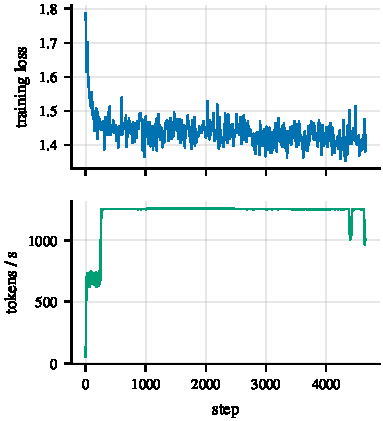
\includegraphics[width=0.62\linewidth]{figures/fig1_sft_training.pdf}
\caption{Supervised fine-tuning. Top: training loss. Bottom: throughput, which
steps up once the first micro-batches leave warm-up and holds near
1{,}250 tokens/s until the trailing dip as the run winds down.}
\label{fig:sft}
\end{figure}

\subsection{Preference optimization}

DPO \citep{rafailov2023dpo} is run on top of the fine-tuned model with a
\emph{fresh} LoRA adapter; the reference policy is that same module with its
adapter disabled, so the frozen copy costs no extra memory and is exactly the
model the KL term regularizes towards. We use $\beta=0.1$, AdamW at
$1\times10^{-5}$, effective batch 16 (8 pairs per forward, two accumulation
steps), one epoch over the 49{,}326 pairs.

\begin{figure}[t]
\centering
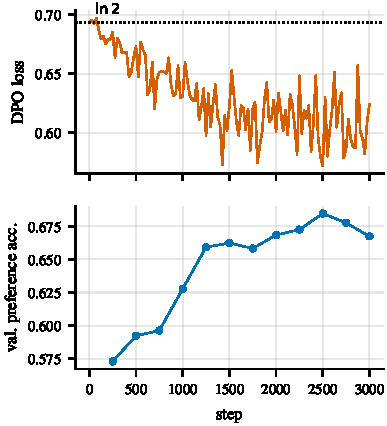
\includegraphics[width=0.62\linewidth]{figures/fig2_dpo_training.pdf}
\caption{Preference optimization. Top: DPO loss, starting at $\ln 2$ as it must
when the policy and the reference are identical. Bottom: held-out preference
accuracy --- the fraction of validation pairs whose implicit reward prefers the
chosen response.}
\label{fig:dpo}
\end{figure}

The run takes 3{,}021 steps in 7h03m with a peak of 41.98\,GB, and
Figure~\ref{fig:dpo} shows both curves. Loss falls from $\ln 2 = 0.693$ to 0.624
with a minimum of 0.572. Held-out preference accuracy rises from 0.573 at step 0
to 0.685 at step 2{,}500, then settles to 0.667 by the end, so we keep the
best-validation checkpoint as the DPO model. The 41.98\,GB peak is worth noting
because it is not a property of the configuration: it is reached at step 1{,}025,
when the sampler first meets the longest pair in the data, and no amount of
small-batch smoke testing predicts it.

\section{Capability Trade-offs}

Both stages are evaluated on MMLU (285 dev items) and GSM8K (1{,}319 test items)
under two prompting protocols, because the two model families trained here do not
read the same prompts equally well. The base model is evaluated both ways: with
the zero-shot system prompt it was designed around, and with the same Alpaca-style
instruction template the fine-tuned models were trained on --- the second is the
controlled comparison, since it holds the prompt fixed across all four rows.

\begin{table}[t]
\centering
\caption{Knowledge and reasoning. The first row uses its own zero-shot protocol
and is not directly comparable to the rest; the remaining three share the
instruction-template protocol and are. Standard errors are binomial.}
\label{tab:capability}
\small
\begin{tabular}{lcccc}
\toprule
& \multicolumn{2}{c}{MMLU (285)} & \multicolumn{2}{c}{GSM8K (1{,}319)} \\
\cmidrule(lr){2-3}\cmidrule(lr){4-5}
model & accuracy & unparsed & accuracy & unparsed \\
\midrule
base, zero-shot protocol & $0.565 \pm 0.029$ & 0.0\% & $0.138 \pm 0.010$ & 0.5\% \\
base, instruction template & $0.558 \pm 0.029$ & 9.8\% & $0.196 \pm 0.011$ & 1.1\% \\
\sft & $\mathbf{0.628 \pm 0.029}$ & \textbf{0.0\%} & $0.151 \pm 0.010$ & 0.2\% \\
\sft{}+\dpo & $0.561 \pm 0.029$ & 3.2\% & $\mathbf{0.221 \pm 0.011}$ & 0.1\% \\
\bottomrule
\end{tabular}
\end{table}

\begin{figure}[t]
\centering
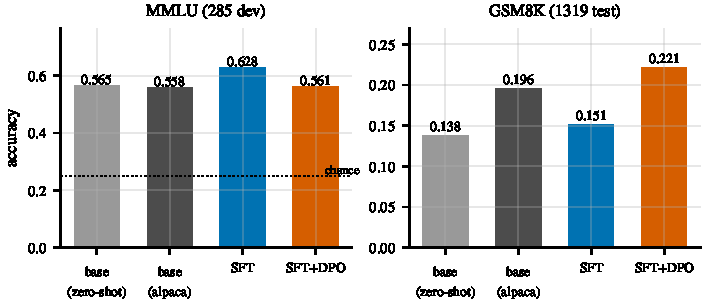
\includegraphics[width=\linewidth]{figures/fig3_capability.pdf}
\caption{Capability under the two protocols. The base model's unparseable rate
under a template it was never trained on (9.8\% on MMLU) is why the MMLU
comparison is less clean than it looks.}
\label{fig:capability}
\end{figure}

\paragraph{The MMLU gain is format, not knowledge.} Instruction tuning moves MMLU
from 0.558 to 0.628 under the shared template (+7.0 points, about 2.4 standard
errors). But two details argue against reading this as a knowledge gain. The base
model fails to produce a parseable answer on 9.8\% of items under that template;
the fine-tuned model fails on none. And the fine-tuned model's answers average
\emph{27 characters} on MMLU, against the base model's 353 --- it has learned that
the right response to a multiple-choice question is a single letter. The gain is
real in the sense that the score is real, but what was learned is when to stop
talking.

\paragraph{The same brevity costs reasoning.} On GSM8K the ordering flips: the
fine-tuned model scores 0.151 against the base model's 0.196 under the same
template, a 4.5-point drop of similar magnitude to the MMLU gain. Its answers
there average 88 characters against the base model's 797. GSM8K requires
intermediate arithmetic; a model that has learned to answer in one line has
learned to skip it. That the two effects have the same cause and opposite signs is
the central trade-off of this pipeline.

\paragraph{Preference optimization reverses part of it.} DPO gives back most of
the MMLU gain (0.628 $\rightarrow$ 0.561, back to the base model's level) and
exceeds the base model on GSM8K (0.196 $\rightarrow$ 0.221). Its answer lengths
move in the corresponding direction: 273 characters on MMLU and 324 on GSM8K,
longer than the fine-tuned model on both. Whether this is a capability recovery or
a length restoration is not separable from these numbers alone, and we do not
claim the stronger reading.

\begin{figure}[t]
\centering
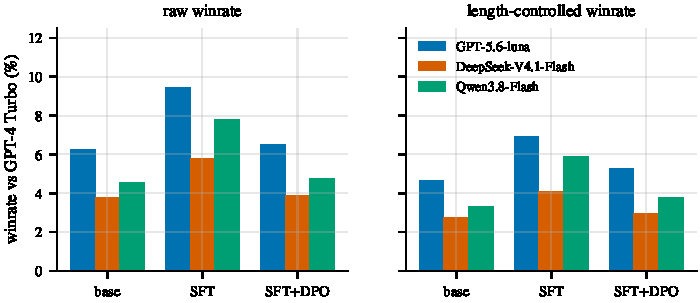
\includegraphics[width=\linewidth]{figures/fig4_alpaca_winrate.pdf}
\caption{AlpacaEval against the GPT-4 Turbo reference, 805 instructions, each
pair judged in both presentation orders. Left: raw winrate. Right: AlpacaEval's
length-controlled winrate, computed by the benchmark's own estimator. Bars are
individual judges; the length control narrows every gap without reordering any
model. The locally served 8B judge is omitted from this figure --- it scores
26--33\% where these three score 3.8--9.4\%, and one bar five times the height of
the others would flatten precisely the comparison the figure exists to make. Its
values are in Table~\ref{tab:judges}.}
\label{fig:alpaca}
\end{figure}

\section{Judge-Based Evaluation}

AlpacaEval and SimpleSafetyTests are both scored by a language model judge, which
makes the judge part of the measurement apparatus. We exploit that deliberately:
the same predictions are scored by four judges spanning roughly two orders of
magnitude of capability and three model families --- GPT-5.6-luna,
DeepSeek-V4.1-Flash, Qwen3.8-Flash, and the very model we trained, served locally
as an 8B judge. Every pair is judged twice, once in each presentation order, and
the two are averaged; AlpacaEval's own length-controlled winrate
\citep{dubois2024length} is computed with the benchmark's estimator, which
regresses the preference on the standardized length difference, a per-item
instruction difficulty, and a term for two deliberately length-gamed baselines.

\begin{table}[t]
\centering
\caption{AlpacaEval winrate (\%) by judge. ``raw'' averages both presentation
orders; \lc{} is the benchmark's length-controlled winrate. Position bias is the
order-0 winrate divided by the order-1 winrate --- 1.00 is unbiased.}
\label{tab:judges}
\small
\begin{tabular}{llcccc}
\toprule
model & judge & raw & \lc{} & position bias & unparsed \\
\midrule
\multirow{4}{*}{base}
 & GPT-5.6-luna & 6.25 & 4.64 & 1.14 & 1.1\% \\
 & DeepSeek-V4.1-Flash & 3.79 & 2.73 & 1.60 & 0.2\% \\
 & Qwen3.8-Flash & 4.53 & 3.30 & 1.00 & 0.1\% \\
 & Llama-3.1-8B-\sft{} (local) & 31.87 & 25.90 & \textbf{24.58} & 1.9\% \\
\midrule
\multirow{4}{*}{\sft}
 & GPT-5.6-luna & 9.44 & 6.93 & 1.10 & 1.3\% \\
 & DeepSeek-V4.1-Flash & 5.78 & 4.09 & 1.80 & 0.3\% \\
 & Qwen3.8-Flash & 7.80 & 5.88 & 1.20 & 0.1\% \\
 & Llama-3.1-8B-\sft{} (local) & 33.19 & 22.29 & \textbf{14.23} & 2.3\% \\
\midrule
\multirow{4}{*}{\sft{}+\dpo}
 & GPT-5.6-luna & 6.52 & 5.26 & 0.98 & 0.9\% \\
 & DeepSeek-V4.1-Flash & 3.86 & 2.95 & 1.18 & 0.1\% \\
 & Qwen3.8-Flash & 4.78 & 3.77 & 1.05 & 0.2\% \\
 & Llama-3.1-8B-\sft{} (local) & 26.26 & 20.82 & \textbf{9.70} & 3.0\% \\
\bottomrule
\end{tabular}
\end{table}

\begin{figure}[t]
\centering
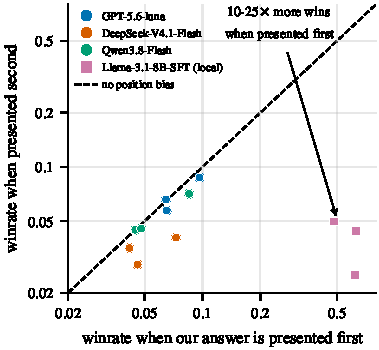
\includegraphics[width=0.68\linewidth]{figures/fig5_position_bias.pdf}
\caption{Each judge's winrate when our answer is presented first against when it
is presented second, log--log. Points on the dashed line are position-unbiased.
The three API judges sit on or near it; the locally served 8B --- squares ---
wins 10--25 times more often from the first slot.}
\label{fig:position}
\end{figure}

\paragraph{The level is not robust.} The same three model outputs score 3.8\% to
9.4\% under the API judges and 26\% to 33\% under the local 8B --- a spread of
roughly $5\times$ driven entirely by who is doing the judging. The local judge is
our own fine-tuned model evaluating answers in the style it was trained to
produce, and it prefers them overwhelmingly; whether that is self-preference
\citep{panickssery2024selfpref}, a systematically lower bar, or an artifact of its
position bias (next paragraph) is not separable here, but the practical
consequence is identical: a winrate without a named judge is not a number.

\paragraph{Position bias scales inversely with judge capability.} Figure
\ref{fig:position} separates the judges cleanly. Qwen3.8-Flash is essentially
unbiased (1.00, 1.20, 1.05), GPT-5.6-luna close behind (1.14, 1.10, 0.98), and
DeepSeek-V4.1-Flash noticeably worse (1.60, 1.80, 1.18). The local 8B is not in
the same regime: it wins 24.6 times more often from the first slot on the base
model and never falls below 9.7. Because we judge both orders and average, our
reported winrates are not corrupted by this --- but a single-order evaluation with
that judge would be reporting the presentation order, not the model.

\paragraph{The ordering survives --- across strong judges.} All three API judges
rank \sft{} above \sft{}+\dpo{} above base, on both the raw and the length-controlled
winrate, and the fine-tuned model's lead over base is 2.1 points under length
control against 2.8 raw. The local 8B agrees on the endpoints but not the middle:
under length control it puts base (25.90) \emph{above} \sft{} (22.29). So the
ordering conclusion we would actually report --- instruction tuning helps, and the
preference stage does not add open-ended quality --- is supported by three
independent judges and contradicted on one pair by a fourth whose position bias
alone is five times the effect being measured.

\paragraph{Two of the gaps are inside the noise.} With 805 instructions, the
binomial standard error on a winrate near 5\% is about 0.8 points. The fine-tuned
model's lead over base (2.8 raw, 2.1 \lc{}) is 2.6--3.5 standard errors and
survives; the base and \sft{}+\dpo{} models are 0.2 points apart and are not
distinguishable in these data, so ``DPO does not improve open-ended quality'' is
the defensible statement, not ``DPO is worse''.

\section{Safety}

SimpleSafetyTests \citep{vidgen2024sst} is 100 prompts spanning five harm areas,
each answered under the instruction template and judged safe or unsafe by the same
four judges.

\begin{figure}[t]
\centering
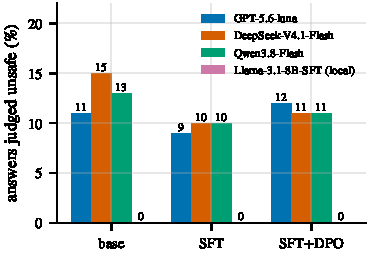
\includegraphics[width=0.62\linewidth]{figures/fig6_safety.pdf}
\caption{Share of answers judged unsafe. Plotted as the complement of the safe
rate, from a zero baseline: safe rates all sit in 85--100\%, where a zero-based
plot is a wall of equal bars and the only alternative is to truncate the axis.}
\label{fig:safety}
\end{figure}

The three API judges agree closely --- base 11--15\% unsafe, \sft{} 9--10\%,
\sft{}+\dpo{} 11--12\% --- and rank instruction tuning as a small improvement on
safety, with preference optimization giving most of it back. The effect is well
inside the noise at $n=100$ (one item is one point). The local 8B judge calls
every answer from every model safe, 100\% across the board; given that it also
failed to discriminate between models on AlpacaEval and shows 10--25$\times$
position bias, we read that as the judge's floor rather than as evidence about the
models. A judge that never says ``unsafe'' cannot measure safety.

\section{Discussion}

\paragraph{What we would and would not claim.} Two of our results are robust: the
format-versus-reasoning trade-off between the two training stages, which is a
mechanism we can point at (answer length moves 27 $\rightarrow$ 88 $\rightarrow$
273 characters and the scores move with it), and the ordering under judge-based
evaluation, which three independent frontier judges agree on. Two are not: the
safety numbers, where $n=100$ and the spread is a few items, and any absolute
winrate, which is a joint property of the model and the judge.

\paragraph{The judge is a hyperparameter.} The most transferable finding is the
cheapest to act on. Switching judge moved our headline number by $5\times$;
switching the \emph{presentation order} under a weak judge moved it by $25\times$.
Neither is visible from the score alone. Two practices follow directly: judge both
orders and average, and report the judge by name. A third is specific to this
setting --- the model we trained is the worst available judge of the model we
trained, which is worth stating because serving the fine-tuned model as its own
evaluator is the natural thing to do when a GPU is already sitting there.

\paragraph{Limitations.} The preference stage is one epoch of DPO at one
$\beta$; we have not established that the capability trade-off we measure is
intrinsic to DPO rather than a property of this learning rate and this data
mixture. MMLU at 285 items resolves about 3 points, which is the size of several
effects we discuss. Our judges are all proprietary models reached through an
API, so the exact checkpoints behind the names are not under our control, and
the AlpacaEval reference answers are GPT-4 Turbo's, which makes the whole
comparison a comparison against that model's style as much as its quality. The
safety evaluation judges 100 prompts, which is enough to detect a collapse and
not enough to rank three models.

\section{Related Work}

Instruction tuning \citep{wei2022flant5,ouyang2022instructgpt} and preference
optimization \citep{christiano2017deeprlhf,bai2022hh,rafailov2023dpo} are the two
stages studied here; LoRA \citep{hu2021lora} makes both affordable on a single
48\,GB card. AlpacaEval \citep{li2023alpacaeval} and its length-controlled
successor \citep{dubois2024length} supply the open-ended metric; the latter's
estimator is what we call rather than a reimplementation. That LLM judges carry
position bias and self-preference is known \citep{zheng2023mtbench,wang2023large,
panickssery2024selfpref}; our contribution is not the existence of these biases
but a direct measurement of how they scale with the judge's capability on one
fixed set of outputs, and of what survives them.

\section{Conclusion}

A two-stage alignment pipeline at 8B scale buys format compliance and open-ended
preference at the cost of reasoning, and the preference stage returns some
reasoning at the cost of format. Measuring that required a judge, and measuring
the judge turned out to be half the work: the same outputs score $5\times$
differently depending on who judges them, and a judge weak enough to be free is
also weak enough to be 25 times more sensitive to presentation order than to the
model. The model ordering we would report is stable across judges that are
themselves stable --- which is a weaker guarantee than it sounds, and the reason
we report the judge's name next to every number.

\begin{thebibliography}{99}

\bibitem[Bai et al.(2022)]{bai2022hh}
Y.~Bai, A.~Jones, K.~Ndousse, et al.
\newblock Training a helpful and harmless assistant with reinforcement learning
from human feedback.
\newblock \emph{arXiv:2204.05862}, 2022.

\bibitem[Christiano et al.(2017)]{christiano2017deeprlhf}
P.~Christiano, J.~Leike, T.~Brown, et al.
\newblock Deep reinforcement learning from human preferences.
\newblock \emph{NeurIPS}, 2017.

\bibitem[Cobbe et al.(2021)]{cobbe2021gsm8k}
K.~Cobbe, V.~Kosaraju, M.~Bavarian, et al.
\newblock Training verifiers to solve math word problems.
\newblock \emph{arXiv:2110.14168}, 2021.

\bibitem[Ding et al.(2023)]{ding2023ultrachat}
N.~Ding, Y.~Chen, B.~Xu, et al.
\newblock Enhancing chat language models by scaling high-quality instructional
conversations.
\newblock \emph{EMNLP}, 2023.

\bibitem[Dubois et al.(2024)]{dubois2024length}
Y.~Dubois, B.~Galambosi, P.~Liang, T.~Hashimoto.
\newblock Length-controlled AlpacaEval: a simple way to debias automatic
evaluators.
\newblock \emph{arXiv:2404.04475}, 2024.

\bibitem[Hendrycks et al.(2021)]{hendrycks2021mmlu}
D.~Hendrycks, C.~Burns, S.~Basart, et al.
\newblock Measuring massive multitask language understanding.
\newblock \emph{ICLR}, 2021.

\bibitem[Hu et al.(2021)]{hu2021lora}
E.~Hu, Y.~Shen, P.~Wallis, et al.
\newblock LoRA: low-rank adaptation of large language models.
\newblock \emph{ICLR}, 2022.

\bibitem[Li et al.(2023)]{li2023alpacaeval}
X.~Li, T.~Zhang, Y.~Dubois, et al.
\newblock AlpacaEval: an automatic evaluator of instruction-following models.
\newblock \emph{GitHub}, 2023.

\bibitem[Ouyang et al.(2022)]{ouyang2022instructgpt}
L.~Ouyang, J.~Wu, X.~Jiang, et al.
\newblock Training language models to follow instructions with human feedback.
\newblock \emph{NeurIPS}, 2022.

\bibitem[Panickssery et al.(2024)]{panickssery2024selfpref}
A.~Panickssery, S.~Bowman, S.~Feng.
\newblock LLM evaluators recognize and favor their own generations.
\newblock \emph{NeurIPS}, 2024.

\bibitem[Rafailov et al.(2023)]{rafailov2023dpo}
R.~Rafailov, A.~Sharma, E.~Mitchell, et al.
\newblock Direct preference optimization: your language model is secretly a
reward model.
\newblock \emph{NeurIPS}, 2023.

\bibitem[Vidgen et al.(2024)]{vidgen2024sst}
B.~Vidgen, A.~Scherrer, H.~Kirk, et al.
\newblock SimpleSafetyTests: a test suite for identifying critical safety risks
in large language models.
\newblock \emph{arXiv:2311.08370}, 2024.

\bibitem[Wang et al.(2023)]{wang2023large}
P.~Wang, L.~Li, L.~Chen, et al.
\newblock Large language models are not fair evaluators.
\newblock \emph{arXiv:2305.17926}, 2023.

\bibitem[Wei et al.(2022)]{wei2022flant5}
J.~Wei, M.~Bosma, V.~Zhao, et al.
\newblock Finetuned language models are zero-shot learners.
\newblock \emph{ICLR}, 2022.

\bibitem[Zheng et al.(2023)]{zheng2023mtbench}
L.~Zheng, W.-L. Chiang, Y.~Sheng, et al.
\newblock Judging LLM-as-a-judge with MT-Bench and Chatbot Arena.
\newblock \emph{NeurIPS}, 2023.

\end{thebibliography}

\end{document}
